\documentclass[a4paper]{scrartcl}

\def \mySubject {Fahrzeugeinsatzplaung}
\def \myTitle {Entwicklung einer Anwendung zur Optimierung}
\def \mySubtitle {}
\def \myAuthor {Oliver Pohling, David Mittelst\"{ä}dt, Henrik Vo\ss}
\def \myDate {15. Juli 2014}

% Seitenabstände und Kopf-/ Fußzeile
\usepackage
[
	left=3.5cm,
	right=2.0cm,
	top=2.0cm,
	bottom=2.0cm,
	includeheadfoot
]{geometry}

%Verweise im PDF
\usepackage{hyperref}

%Schoene Verweise
\usepackage[german]{fancyref}

% Deutsche Begriffe
\usepackage{polyglossia}
\setdefaultlanguage[spelling=new, babelshorthands=true]{german}

%Graphiken einbinden
\usepackage{graphicx} 

% Weitere Tabellen Funktionen
\usepackage{tabularx}

% Macht das Label "`LastPage"' auf die letzte Seite.
\usepackage{lastpage}

% Literatur-Verzeichniss nach DIN 1505
\usepackage[numbers]{natbib}

% Horizontale Linien
\usepackage{booktabs}

% Mehrere Bilder nebeneinander
\usepackage{subfigure}

\usepackage[section]{placeins}

\usepackage{pgfplots}
\pgfplotsset{compat=1.9}


\usepackage{scrpage2}
\pagestyle{scrheadings}
\ihead{\mySubject}
\chead{ }
\ohead{\myDate}
\ifoot{\myAuthor }
\cfoot{ }
\ofoot{Seite \thepage~von~\pageref{LastPage}}


% Kein Einrücken beim Absatz, dafür eine halbe Zeile Abstand
\setlength\parindent{0pt}
\setlength\parskip{6pt}


%%%%%%%% Tabellen

\subject{\mySubject}
\title{\myTitle}
\subtitle{\mySubtitle}
\author{\myAuthor}
% Stellt ein Bild mit Label und Caption dar.
%
% Parameter:
% #1: Größe (optional)
% #2: Label
% #3: Dateiname
% 4#: Caption
\newcommand{\myfigure}[4][width=0.95\textwidth]{
  \begin{figure}[ht!]
    \begin{center}
      \includegraphics[#1]{#3}
      \caption{#4}
      \label{fig:#2}
    \end{center}
  \end{figure}
}

% Stellt zwei Bilder nebeneinander dar.
% Die gesamte Figure kann mit fig:#1 referenziert werden.
% Die linke Figure kann mit fig:#1_l und die rechte mit fig:#1_r referenziert werden.
%
% Parameter:
% #1: Gesamtes Label
% #2: Gesamte Caption
% #3: Dateiname links
% #4: Größe links
% #5: Caption links
% #6: Dateiname rechts
% #7: Größe rechts
% #8: Caption rechts
\newcommand{\twoFigures}[8]{
  \begin{figure}[ht!]
    \begin{center}
      \subfigure[#5]{
	\label{fig:#1_l}
	\includegraphics[#4]{#3} 
      }
      \hspace{0.5cm}
      \subfigure[#8]{
	\label{fig:#1_r}
	\includegraphics[#7]{#6} 
      }
      \caption{#2}
      \label{fig:#1}
    \end{center}
  \end{figure}
}


% Gibt eine Einheit einheitlich aus.
%
% Parameter:
% #1: Einheit die einheitlich ausgegeben werden soll.
\newcommand{\einheit}[1]{
  \textit{[#1]}
}
 
\newcommand{\processlist}[3][\relax]{% 
  \def\listfinish{#1}% 
  \long\def\listact{#2}% 
  \processnext#3\listfinish} 
\newcommand{\processnext}[1]{% 
  \ifx\listfinish#1\empty\else\listact{#1}\expandafter\processnext\fi} 
  
\newcommand{\TODO}[1]{\textbf{\textit{TODO(#1)}}}


\begin{document}
\maketitle

\begin{abstract}
  Was für ein Projekt!
\end{abstract}

\newpage
\tableofcontents

\newpage

\section{Einleitung}
\subsection{Einführung}
Ziel dieses Projektes ist es, ein Programm zu entwickeln, mit dem eine Fahrzeugeinsatzplanung unter Berücksichtigung bestimmter Restriktionen durchgeführt werden kann. 

% TODO Beschreiben was die Fahrzeugeinsatzplanung ist?

\subsection{Anforderungen}
\label{sec:Anforderungen}
Dem Programm wird eine Konfiguration übergeben, in der folgende Parameter beschrieben sind:
\begin{itemize}
 \item Fahrzeuge
 \begin{itemize}
  \item Ein Fahrzeug kann ein Produkt transportieren
  \item Durchschnittliche Geschwindigkeit
  \item Kapazität (maximale Anzahl der Produkte)
  \item Zeitfenster (Arbeitsbeginn und -ende)
  \item Start- und End-Depot (Station)
 \end{itemize}
 \item Produkte
 \begin{itemize}
  \item Name des Produkts
 \end{itemize}
 \item Station
 \begin{itemize}
  \item Name der Station
  \item X-Y-Koordinaten
 \end{itemize}
 \item Auftrag
 \begin{itemize}
  \item Name des Auftrages
  \item Zu transportierendes Produkt
  \item Anzahl der Produkte
  \item Beliebige Auf- und Ablade-Station
  \item Zeitfenster bei Auf- und Ablade-Station
 \end{itemize}
\end{itemize}
Die Entfernung zwischen den Stationen kann über die Koordinaten berechnet werden. 

\subsection{Restriktionen}
\label{sec:Restriktionen}
Folgende Restriktionen sind bei der Planung zu berücksichtigen:
\begin{itemize}
 \item Alle Aufträge müssen erledigt werden.
 \item Ein Fahrzeug darf nicht überladen werden.
 \item Ein Fahrzeug startet und endet im Depot.
 \item Ein Fahrzeug darf nur innerhalb seines Zeitfensters fahren.
 \item Ein Produkt muss zuerst aufgeladen werden, bevor es abgeladen werden kann.
 \item Das Auf- und Abladen muss innerhalb des Zeitfensters erfolgen.
\end{itemize}

\section{GenetischerAlgorithmus}
Das nachfolgende Kapitel stellt den genetischen Algorithmus, als Verfahren zur Lösung komplexer Optimierungsprobleme, vor. Dazu werden im ersten Schritt die benötigten Grundlagen geschaffen und im Anschluss die speziellen Operatoren im Zusammenhang mit dem "`PDPTW"' vorgestellt. 

\subsection{Grundlagen}
Bei den genetischen Algorithmen handelt es sich um Verfahren, die zur Lösung komplexer Optimierungsaufgaben eingesetzt werden. Sie beruhen auf Methoden und Erkenntnisse der biologischen Genetik. Dabei dient insbesondere die Evolutionstheorie als Vorbild für die Entwicklung der genetischen Algorithmen, da die Evolution bislang gute Ergebnisse in der Natur geliefert hat. 

Die grundlegende Arbeit, zur Schaffung dieser Verfahrenstechnik, wurde von I. Rechenberg mit dem 1960 erschienenen Werk "`Evolutionsstrategie"' geschaffen. Auf diesem Wissen aufbauend, erfand John Holland 1975 die genetischen Algorithmen, die in seinem Werk "`Adaption in Natural and Artificial Systems"' niedergeschrieben wurden.

Der genetische Algorithmus beruht dabei auf eine simple Verfahrenstechnik, welche nachfolgend dargestellt und erklärt wird:
\begin{itemize}
 \item Initialisiere Population P
 \item Evaluiere alle Individuen in P
 \item Wiederhole, solange Abbruchbedingung nicht erreicht
 \begin{itemize}
  \item Selektiere ein Individuenpaar x, y aus P als Eltern
  \item Erzeuge zwei Nachkommen x‘, y‘ aus x und y durch Anwendung von Crossover-Operationen mit der Wahrscheinlichkeit p(cross)
  \item Erzeuge modifizierte Nachkommen x‘‘, y‘‘ aus x‘ und y‘ durch Anwendung von Mu\-ta\-tions-Operatoren mit der Wahrscheinlichkeit p(mut)
  \item Füge x‘‘ und y‘‘ der Population P hinzu und entferne schlechtere Individuen
 \end{itemize}
 \item Gib das beste Individuum aus P als Lösung aus.
\end{itemize}

Die einzelnen Schritte des genetischen Algorithmus werden dabei in den nachfolgenden Kapiteln anhand einer speziellen Problemstellung (PDPTW) konkretisiert und erläutert.

\subsection{Repräsentation}
Eine der größten Herausforderungen für die Entwicklung und den Erfolg des genetischen Algorithmus ist die Wahl einer geeigneten Repräsentationsebene. Dazu weißt der PDPTW zwei strukturell heterogene Teilprobleme auf. Zum einen muss eine Zusammenfassung von Aufträgen mit ihrer Zuordnung zu einem Fahrzeug als Gruppierungsproblem dargestellt werden. Auf der anderen Seite ist zusätzlich ein Reihenfolgeproblem zu lösen, indem eine zulässige Route bestimmt wird, in der die Ladeorte anzufahren sind. Aus diesen Einschränkungen folgt, dass beispielsweise eine binäre Kodierung, die im klassischen genetischen Algorithmus angewandt wird, keine geeignete Repräsentationsform darstellt. 

Bevor nun eine Möglichkeit der Darstellung der beiden genannten Aspekte vorgestellt wird, müssen die Begriffe des Individuums und des Gens in den Kontext des PDPTW gebracht werden. Ein Individuum ist im nachfolgenden ein kompletter Tourenplan, der aus der Gesamtheit aller Touren besteht, die zur Erfüllung aller Aufträge notwendig sind. Ein Gen hingegen besteht aus exakt einer Tour, der ein Fahrzeug und die verschiedene Aufträge zugeordnet sind. Dies soll die nachfolgende \Fref{fig:Repraesentation1} verdeutlichen:

\myfigure[]{Repraesentation1}{Repraesentation1.pdf}{} % TODO Bildunterschrift

Hier ist im unteren linken Bereich das verwendete Fahrzeug (Fahrzeug 5) zu finden, das für die Auslieferung der Aufträge 1, 3 und 4 verantwortlich ist. Desweiteren soll im späteren Verlauf zusätzlich die Reihenfolge identifizierbar sein, um genau zu wissen, wann welcher Auftrag ab- bzw. aufgeladen wurde. Ein Individuum stellt demnach die Gesamtheit aller Touren dar, die zur Erledigung aller Aufräge gebildet werden müssen. Dies verdeutlich die \Fref{fig:Repraesentation234}:

\begin{figure}[ht!]
	\centering
      \subfigure[sd]{  % TODO Bildunterschrift
	\label{fig:Repraesentation2}
	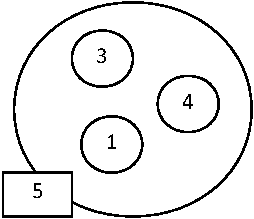
\includegraphics[]{Repraesentation2.pdf} 
      }
      \hspace{0.5cm}
      \subfigure[df]{  % TODO Bildunterschrift
	\label{fig:Repraesentation3}
	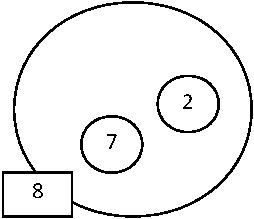
\includegraphics[]{Repraesentation3.pdf} 
      }
      \hspace{0.5cm}
      \subfigure[sd]{  % TODO Bildunterschrift
	\label{fig:Repraesentation4}
	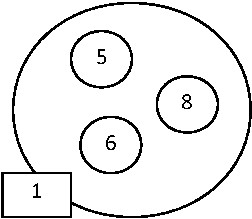
\includegraphics[]{Repraesentation4.pdf} 
      }
      \caption{}  % TODO Bildunterschrift
      \label{fig:Repraesentation234}
\end{figure}

Hierbei handelt es sich um ein konkretes Individuum, das drei Fahrzeuge verwendet, um die gezeigten acht Aufträge zu erfüllen. Zusätzlich muss jedes Gen mit einer ergänzenden Datenstruktur assoziiert werden, so dass im späteren Verlauf der Reihenfolgeaspekt dargestellt werden kann. Diese Darstellung wird im Umfeld des genetischen Algorithmus als Phänotyp bezeichnet. Dies veranschaulicht die \Fref{fig:Repraesentation5} zu einer gegebenen Tour:

\myfigure[]{Repraesentation5}{Repraesentation5.pdf}{} % TODO Bildunterschrift

Auf diese Informationen haben die genetischen Operatoren unmittelbaren Zugriff, um eine möglichst große Varianz in die spätere Population einzubringen.

\subsection{Aufbau der Startpopulation}
Bevor der genetische Algorithmus arbeiten kann, muss im ersten Schritt eine Startpopulation erzeugt werden, die für den Algorithmus als Ausgang dient. Dazu gibt es prinzipiell zwei verschiedene Vorgehensweisen:

\begin{enumerate}
 \item Zufällige Auswahl von Individuen mit zufälligen Merkmalen
 \item Auswahl von "`guten"' Individuen, die durch bestimmte Konstruktionsheuristiken erzeugt wurden
\end{enumerate}

Die zweite Variante bringt ein gewisses Risiko mit, da es beim genetischen Algorithmus passieren kann, dass die Suche, aufgrund bereits guter Lösungen, vorzeitigt konvergiert. Um diesem Problem entgegen zu wirken, wurde der Aufbau der Startpopulation mit beiden Möglichkeiten gekoppelt. Dies soll die  \Fref{fig:Repraesentation6} verdeutlichen:

\myfigure[]{Repraesentation6}{Repraesentation6.pdf}{} % TODO Bildunterschrift

Der Großteil der Population wird dabei zufällig erzeugt, wobei ein ausgewählter Teil sich den Konstruktionsheuristiken bedient. Dabei handelt es sich zum einen um das Nearest-Neighbor- und zum anderen um das Sweep-Verfahren, die in den folgenden Kapiteln kurz vorgestellt werden.

\subsubsection{Nearest-Neighbor}
Beim Nearest-Neighbor handelt es sich um ein bekanntes heuristisches Eröffnungsverfahren was beispielsweise zur Lösung des „Problems des Handlungsreisenden“ verwendet wird. Da das PDPTW eine Abwandlung von dieser Problemstellung ist, eignet sich diese Heuristik ideal für die Erzeugung von potentiellen Startindividuen. Dabei wird bei dieser Technik von einem beliebigen Startpunkt ausgehend der nächstdichteste Knoten besucht. Dies wird sukzessiv fortgesetzt, bis alle Knoten besucht wurden. 

\subsubsection{Sweep}
Der Sweep-Algorithmus bedient sich einer anderen Technik zum Finden des nächstmöglichen Knotens. Hier wird von einem beliebigen Knoten ausgehend, der Knoten gewählt, der den geringsten Winkel von einer definierten Startkante aufweist. Dies kann sowohl im oder entgegengesetzt dem Uhrzeigersinn durchgeführt werden.

\subsection{Individuenauswahl (Selektion)}
\label{sec:Selektion}
Die Selektion bestimmt welche Individuen sich paaren dürfen, und erzeugt aus Ihnen die Menge der Nachkommen. Dabei kann die Auswahl entweder komplett zufällig stattfinden oder ins direkte Verhältnis zur Fitness eines Individuums gesetzt werden. Wenn man sich für eine reine fitnessproportionale Selektion entscheidet, so ist ein verhältnismäßig niedriger Selektionsdruck vorhanden, da der genetische Algorithmus verhältnismäßig lange konvergiert. Abhilfe schafft dort eine Ranglistenbasierte Selektion. Bei diesem Verfahren wird die Selektionswahrscheinlichkeit nicht mehr ins direkte Verhältnis zur Fitness gesetzt. Stattdessen werden die unterschiedlichen Individuen nach ihrer Fitness sortiert, so dass die Tour mit dem besten Ergebnis an oberster Stelle der Population steht. Im nächsten Schritt erfolgt die Auswahl der möglichen Kinder für die oberen Elemente der Rangliste mit einer höheren Wahrscheinlichkeit als tieferliegende Individuen. 

Zusätzlich wird auch hier auf ein Verfahren zurückgegriffen, welches die möglichen Eltern rein zufällig wählt. Dies hat den Vorteil, dass auch Individuen mit schlechter Fitness als potentieller Elternteil gewählt wird. Dadurch werden ggf. mehr genetische Informationen in die nächste Population übertragen und eine zu frühe Konvergenz, aufgrund von sehr guten Fitnesswerten, verhindert. 

Die Kombination der beiden Techniken veranschaulicht die \Fref{fig:Repraesentation7}. Dort wird als mögliches Elternpaar zum einen das Individuum 2 aufgrund der Fitness ausgewählt. Zum anderen wird Individuum 100 rein zufällig gewählt. Dadurch besteht der Vorteil, dass das Individuum, trotz schlechter Fitness, ggf. eine gute Kombination hervorbringt.

\myfigure[]{Repraesentation7}{Repraesentation7.pdf}{} % TODO Bildunterschrift

\subsection{Rekombination (Crossover)}
Bei der Rekombination, auch als Crossover bezeichnet, handelt es sich um den Vorgang, aus zwei Elternpaaren neue Individuen zu erzeugen. Dieses Verfahren stellt dabei einen der wichtigsten Suchoperatoren für genetische Algorithmen dar. Dabei werden die Nachkommen aus den Informationen der gekreuzten Elternpaare systematisch zusammengesetzt. Gesteuert wird der Crossover durch eine Wahrscheinlichkeit, die bestimmt ob entweder nur einfache Kopien der Eltern erzeugt werden, oder ein Operator zur Erzeugung der Nachkommen verwendet wird. Dazu werden nachfolgend zwei verschiedene Varianten vorgestellt.

\subsubsection{Crossover mit Control-String}
Bei dieser Variante der Rekombination wird, auf Grundlage der gewählten Eltern, ein Bit-String gebildet, der letztendlich zu der Entscheidung führt, ob sich der Nachkomme aus einem Teil des ersten oder zweiten Elternteils zusammensetzt. Im Kontext der Fahrzeugeinsatzplanung soll dies die \Fref{tab:CrossoverControlString} verdeutlichen:

\begin{table}[ht!]
 \centering
 \caption{Crossover mit Control-String}
 \begin{tabular}{ll}
  \textbf{Fahrzeug 1 (Plan 1):}	& $1+ \rightarrow 4+ \rightarrow 1- \rightarrow 7+ \rightarrow 7- \rightarrow 4-$ \\
  \textbf{Control-String:} 	& 1 ~ 0 ~ 0 ~ 0 ~ 1 ~ 1 ~ 0 ~ 1 ~ 0 ~ 1 \\
  \textbf{Fahrzeug 1 (Plan 2):} 	& $1+ \rightarrow 5+ \rightarrow 5- \rightarrow 1-$ \\
  \textbf{Nachkomme:} 		& $1+ \rightarrow 5+ \rightarrow 5- \rightarrow 1- \rightarrow 4+ \rightarrow 7+ \rightarrow 7- \rightarrow 4-$
 \end{tabular}
 \label{tab:CrossoverControlString}
\end{table}

Oben und unten ist jeweils eine Tour dargestellt, die jeweils einem Elternindividuum entnommen wurde. In der Mitte befindet sich der "`Control-String"', wobei die Länge der Summe der Aufträge (Be- und Entladung) der beiden Eltern entspricht. Nun nimmt ein Element des Strings zufällig eine Ausprägung von "`1"' oder "`0"' an, wobei die "`1"' besagt, dass das Element aus Fahrzeug 1 von Plan 1 für den Nachkommen gewählt wird. Auf gleiche Weise geschieht dies mit der "`0"' für Fahrzeug 1 aus Plan 2. Bereits gewählte Aufträge werden dabei nicht mehr berücksichtigt. Letztendlich entsteht der unten in der \Fref{tab:CrossoverControlString} aufgeführte Nachkomme.

\subsubsection{Crossover nach Falkenauer}
Die zweite Variante für einen möglichen Crossover orientiert sich an dem gruppenzentrierten Operator, der von Falkenauer vorgeschlagen wurde. Im Wesentlichen besteht er aus vier Phasen die nachfolgend in der \Fref{fig:CrossoverFalkenau} dargestellt und erläutert werden.

\myfigure[width=0.9\textwidth]{CrossoverFalkenau}{CrossoverFalkenau.png}{} % TODO Bildunterschrift

\begin{enumerate}
 \item In der ersten Phase werden in jedem der beiden Eltern zufällig je zwei Crossover-Punkte gebildet, die innerhalb von jedem Elternteil den Anfang und das Ende des Crossover-Segments darstellen.
 \item Hier wird das Crossover-Segment des zweiten Elternteils an den ersten Crossover-Punkt des ersten Elternteils angefügt. Die dazugehörigen Touren werden vom Elternteil unmittelbar übernommen, also vorerst ohne Neukonstruktion. Als Folge kann eine Anzahl von Aufträgen mehreren Fahrzeugeinsatzplänen zugeordnet sein. Desweiteren kann es auch vorkommen, dass mehrere Touren vom gleichen Fahrzeug bedient werden.
 \item In dieser Phase werden alle auftretenden Probleme aus Punkt 2 aufgelöst. Dabei wird so vorgegangen, dass vorerst alle neuerhaltenden Touren unangetastet bleiben und die Touren des empfangenden Elternteils modifiziert werden, um alle Konflikte zu lösen. Dazu werden alle Touren eliminiert, die auf ein Fahrzeug referenzieren, das neu hinzugefügt wurde (im Beispiel Fahrzeug 1). Falls anschließend noch einzelne Aufträge doppelt vorhanden sind, so werden auch diese aus den Touren des empfangenden Elternteils eliminiert (im Beispiel die Aufträge 2, 6 und 7). Nach Abschluss dieser Operation sind einzelne Aufträge (im Beispiel 5 und 8) noch vorerst keiner Tour zugeordnet.
 \item Die verbleibenden Aufträge werden rein zufällig an die vorhandenen Touren vergeben. Dazu kann beispielsweise auch ein komplett neues Fahrzeug allokiert werden. Nach Abschluss von Schritt 4 liegt letztendlich als Ergebnis ein vollständiges Kind vor.
\end{enumerate}

Gegebenenfalls können die Schritte 2-4 mit vertauschten Rollen der Eltern wiederholt werden, falls man ein zweites Kind erzeugen möchte.

\subsection{Mutation}
Unter der Mutation, im Zusammenhang zum Genetischen Algorithmus, versteht man die Art und Weise, um aus einem Elternteil ein neues Individuum durch zufällige Veränderung zu erzeugen. Diese Änderung wird dabei auch hier durch eine Wahrscheinlichkeit gesteuert, die angibt, ob eine Mutation an einem Individuum stattfindet oder nicht. Sie dienen hauptsächlich dazu, eine gewisse Inhomogenität und Divergenz mit in die Population herein zu bringen, was durch die Rekombination unter Umständen nicht möglich ist. Zusätzlich wird eine frühzeitige Konvergenz des Algorithmus verhindert und der Selektionsdruck abgeschwächt. 

Innerhalb dieser Arbeit wurden insgesamt sieben verschiedene Mutationsoperatoren entwickelt, welche mit einer Gewichtung dem genetischen Algorithmus hinzugefügt werden können. Diese werden im nachfolgenden jeweils mit einer Abbildung vorgestellt.

\subsubsection{Aufteilung der längsten Route}
\label{sec:AufteilungLangaesteRoute}
Dieser Operator überprüft die Länge von jeder Tour innerhalb einer Fahrzeugeinsatzplanung. Die Tour, welche die längste Strecke anhand der gefahrenen Kilometer aufweist (im Beispiel Fahrzeug 5), wird entfernt und auf die verbleibenden Touren aufgeteilt (siehe \Fref{fig:MutationAufteilen1} und \Fref{fig:MutationAufteilen2}). Dabei werden die Aufträge rein zufällig an die anderen Touren vergeben.

\myfigure[]{MutationAufteilen1}{MutationAufteilen1.pdf}{Ausgangsindividuum}
\myfigure[]{MutationAufteilen2}{MutationAufteilen2.pdf}{Neues Individuum}

\subsubsection{Aufteilung der kleinsten/zufälligen Tour}
Diese beiden Mutationsoperatoren arbeiten auf die gleiche Weise wie unter \Fref{sec:AufteilungLangaesteRoute} beschrieben. Dabei wird hier der mögliche Kandidat entweder zufällig oder anhand der kleinsten Tour gewählt. Da die Arbeitsweise nahezu identisch ist, wurde hier auf eine zusätzliche Abbildung verzichtet.

\subsubsection{Verschiebung einer/mehrerer Aktion(en) innerhalb einer Tour}
Dieser Operator geht noch einen Schritt weiter und verschiebt innerhalb einer Tour eine Aktion. Bei einer Aktion kann es sich um ein Auf- oder Abladen eines bestimmten Auftrags handeln, was über die assoziierte Datenstruktur zu einer Tour gewährleistet wird. (siehe \Fref{fig:AktionVerschieben}). Ein weiterer Operator verschiebt zusätzlich nicht nur eine Aktion, sondern ganze Subrouten, die in ihren Grenzen zufällig gewählt werden.

\myfigure[]{AktionVerschieben}{AktionVerschieben.pdf}{Verschiebung einer/mehrerer Aktion(en) innerhalb einer Tour}

Die Repräsentation (links in \Fref{fig:AktionVerschieben}) bleibt davon unberührt, da es sich um eine reine Manipulation der Datenstruktur handelt. Konkret wird in diesem Beispiel das Abladen des Auftrags 3 mit dem Aufladen des Auftrags 2 vertauscht. Dies kann zur Folge habe, dass falsche Lösungen entstehen, da nach dem Operator keine Überprüfung und ggf. eine Korrektur stattfindet. Der Umgang mit der genannten Problematik wird jedoch im \Fref{sec:Nachfolgegeneration} erläutert. % TODO Referenz

\subsubsection{Verschiebung von Subtouren über eine Tour hinaus}
Die bisherigen Operatoren haben lediglich ein Gen des Individuums mutiert. Um eine größere Varianz, unter dem Einfluss der Mutation, zu erschaffen wurde zusätzlich eine Möglichkeit entwickelt, wo ein Tauschen von Subtouren zwischen den unterschiedlichen Genen eines Individuums stattfindet. Dies veranschaulicht die \Fref{fig:SubrouteVerschieben}:

\myfigure[]{SubrouteVerschieben}{SubrouteVerschieben.pdf}{Verschiebung von Subtouren über eine Tour hinaus}

Dadurch entstehen letztendlich zwei komplett neue Touren innerhalb einer Fahrzeugeinsatzplanung, wobei diese Mutation Einfluss auf die Repräsentationsebene hat, da beispielsweise die Order 2 und 7 von Tour 2 nun von der Tour 1 ausgeführt wird. 

\subsubsection{Kombination von 2 Touren}
Den letzten genetischen Operator für eine Mutation stellt die Kombination von 2 Touren zu einer neuen Tour dar. Das Fahrzeug, das die Aufträge abliefert, wird zufällig aus den beiden vorhandenen gewählt. Dies wird durch die \Fref{fig:Kombination} veranschaulicht:

\myfigure[]{Kombination}{Kombination.pdf}{Verschiebung von Subtouren über eine Tour hinaus}

\FloatBarrier
~\newpage
\subsection{Bildung der Nachfolgegeneration}
\label{sec:Nachfolgegeneration}
Über die Mechanismen der Selektion hinaus, die in \Fref{sec:Selektion} definiert wurden, wird sowohl die komplette Ausgangspopulation, als auch die neue Population, für die Nachfolgepopulation berücksichtigt. Dazu findet auch an der Neuen wiederum eine Sortierung statt. Zum einen werden alle invaliden Lösungen, d.h. Lösungen, wo beispielsweise ein Ent- vor dem Beladen erfolgt, ans Ende der Population verschoben. Danach erfolgt eine Sortierung anhand der Fitness. Demnach werden beiden Populationen zu einer Nachfolgepopulation der definierten Menge (im Beispiel 100) zusammengefasst. Zur Veranschaulichung dient die \Fref{fig:Nachfolgegeneration}:

\myfigure[scale=0.85]{Nachfolgegeneration}{Nachfolgegeneration.pdf}{Bildung der Nachfolgegeneration}

Das Resultat ist die neue Nachfolgepopulation, die wieder in den genetischen Algorithmus einfließt, bis eine Abbruchbedingung erreicht wird. Diese Verfahrenstechnik hat den Vorteil, dass bereits potentiell gute Lösungen, die in der Ausgangspopulation vorhanden waren, erhalten bleiben und nicht durch die neugebildete Population überschrieben werden.

\FloatBarrier
\subsection{Abbruchbedingung}
Als letzten entscheidenden Punkt muss beim genetischen Algorithmus eine Abbruchbedingung definiert werden, wann die Suche abgeschlossen ist. Dazu wurden zwei Varianten entwickelt:

\begin{enumerate}
 \item Der genetische Algorithmus wird solange durchlaufen, bis eine definierte Anzahl von Iterationen (z.B. 5000) erreicht wurde.
 \item Die Fitness der besten Lösung entspricht einem definierten Abstand von der Durchschnittsfitness von allen Lösungen zu dieser Lösung
\end{enumerate}

Die erste Bedingung wird für den Fall benötigt, dass der genetische Algorithmus nicht unendlich oft durchlaufen wird. Eine Iteration entspricht dabei dem Weg von einer Ausgangspopulation bis hin zu Neubildung der Nachfolgegeneration.

Die zweite Bedingung ist die eigentlich entscheidende, da der Algorithmus solange laufen soll, bis keine bessere Lösung mehr gefunden wird. Ist dies der Fall, so kann die genetische Suche abgeschlossen werden und das erste Individuum in der Population entspricht der optimalen Lösung für eine gegebene Konfiguration.
\section{Softwarearchitektur}

\subsection{Systemdesign}
Das Systemdesign setzt sich im wesentlichen aus den folgenden vier Modulen zusammen:
\begin{enumerate}
 \item Konfigurationsgenerierung
 \item Konstruktionsverfahren
 \item Genetisches Optimierungsverfahren
 \item Ergebnisvisualisierung
\end{enumerate}
Desweiteren sind zwei Datenmodelle definiert:
\begin{enumerate}
 \item Konfiguration-Datenmodell
 \item Ergebnis-Datenmodell
\end{enumerate}

\subsection{Konfigurations-Datenmodell}
Das Konfiguration-Datenmodell beschreibt die Konfiguration, die vom Anwender zur Verfügung gestellt wird. Sie umfasst Stationen, Fahrzeuge, Produkte, Aufträge und Zeitfenster (siehe \Fref{fig:KonfigurationDatenmodell}).

\subsection{Ergebnis-Datenmodell}
\myfigure[width=0.95\textwidth]{ErgebnisDatenmodell}{../src/main/java/de/hsbremen/kss/model/Model.png}{Repräsentation eines Plans mit Touren und Aktionen}

\subsection{Konfigurationsgenerierung}

\subsection{Genetischer Algorithmus}
\myfigure[width=0.95\textwidth]{KonfigurationDatenmodell}{../src/main/java/de/hsbremen/kss/genetic/GeneticAlgorithm.png}{Klassendiagramm vom genetischen Algorithmus}
\section{Umsetzung}

\subsection{Verwendete Bibliotheken}
Im Rahmen der Entwicklung wurden diverse OpenSource - Bibliotheken eingeführt, um die Entwicklung zu beschleunigen und die Qualität der Software zu steigern. Im folgenden werden die verwendeten Bibliotheken beschrieben:
\begin{description}
 \item[Apache Commons Math] (Version 3.2, Apache License 2.0) \cite{apache:CommonsMath} Stellt mathematische Funktionen zur Verfügung. Wird unteranderem für die Berechnung der Entfernungen verwendet.
 \item[Apache Commons Lang] (Version 3.3.1, Apache License 2.0) \cite{apache:CommonsLang} % TODO wird es wirklich verwendet?
 \item[Apache Commons Collections] (Version 4.0, Apache License 2.0) \cite{apache:CommonsCollection} Erweitert das Java-Collec\-tions-Framework. 
 \item[Joda-Time] (Version 2.3, Apache License 2.0) \cite{joda:jodatime} % TODO wird es wirklich verwendet?
 \item[JUnit] (Version 4.11, Eclipse Public License) \cite{junit:junit} JUnit ist die Standard-Bibliothek für Unit-Tests unter Java. 
 \item[Hamcrest] (Version 1.3, BSD 3-Clause) \cite{hamcrest:hamcrest} Mit Hamcrest ist es möglich bei Tests "`sprechendere"' Ausdrücke zu formulieren.
 \item[EasyMock] (Version 3.2, Apache License 2.0) \cite{easymock:easymock} EasyMock ermöglicht ein einfaches Erstellen von Mock-Objekten für den Unit-Test.
 \item[Simple Logging Facade for Java (SL4J)] (Version 1.7.6, MIT license) \cite{qos:slfj} SLF4J ist eine Log\-ging-Schnittstelle und wird zur Ausgabe auf der Konsole verwendet.
 \item[Logback] (Version 1.1.1, Eclipse Public License v1.0 und LGPL 2.1) \cite{qos:logback} Wird als Implementierung für SLF4J eingesetzt.
 \item[Google Guave] (Version 17.0, Apache License 2.0) \cite{google:guave} Guave ist eine Sammlung von Softwarebibliotheken. Es wird ausschließlich der EventBus für die Kommunikation zwischen den Softwarekomponenten verwendet.
 \item[JFreeChart] (Version 1.0.17, LPGL) \cite{ObjectRefineryLimited:JFreeChart} JFreeChart wird zur Darstellung der Graphen verwendet.
\end{description}

% TODO Entwicklungsumgebung beschreiben?

\subsection{Mutation}
\myfigure[width=0.95\textwidth]{Mutation}{../src/main/java/de/hsbremen/kss/genetic/mutation/Mutation.png}{Implementierte Mutationsalgorithmen}

\subsection{Grafische Oberfläche}

\myfigure[width=0.95\textwidth]{FitnessDistribution}{FitnessDistribution.png}{Verteilung des Fitnesswertes} % TODO Bildunterschirft
\myfigure[width=0.95\textwidth]{FitnessLengthGraph}{FitnessLengthGraph.png}{} % TODO Bildunterschirft
\myfigure[width=0.95\textwidth]{Map}{Map.png}{} % TODO Bildunterschirft



\section{Experimente}
In den Experimenten wird der genetische Algorithmus auf seine Funktionsweise überprüft. Außerdem soll der Einfluss der Änderungen der Parameter der Komponenten auf das Ergebnis des Algorithmus untersucht werden. Zuerst wird hierfür eine Zielsetzung definiert. Darauf folgen dann eine Beschreibung der verwendeten Konfiguration für die Experimente, die Durchführung sowie eine Auswertung zum Abschluss dieses Kapitels.

\subsection{Zielsetzung}
\label{sec:Zielsetzung}
Mit Hilfe der Experimente soll festgestellt werden, ob der genetische Algorithmus das erwartete Verhalten, sukzessive Verbesserung der Individuen, aufweist. Wie bereits in den vorherigen Kapiteln beschrieben, besteht der genetische Algorithmus aus verschiedenen Komponenten. Die Funktionsweise einzelner Komponenten wurde bereits mit Unittests nachgewiesen. In den nachfolgenden Experimenten soll nun das Zusammenspiel dieser Komponenten beobachtet werden sowie deren Auswirkung auf das Ergebnis des genetischen Algorithmus. Dabei spielen folgende Bestandteile des genetischen Algorithmus eine zentrale Rolle:
\begin{itemize}
 \item Mutationen
 \item Selektion
 \item Crossover
 \item Fitnesstest
\end{itemize}
An diesen Bestandteilen werden während der Experimente Veränderungen vorgenommen und die Auswirkungen auf das Ergebnis untersucht.

Um die Qualität eines Ergebnisses beschreiben zu können, müssen vor den Experimenten Indikatoren festgelegt werden. Für die hier durchgeführten Experimente werden folgende Indikatoren verwendet:
\begin{itemize}
 \item Länge eines Plans
 \item Anzahl der Fahrzeuge
 \item Anzahl der Iterationen
 \item Anzahl und Art der Restriktionsverletzungen
\end{itemize}
Als Indikator hätte auch der Fitnesswert dienen können, allerdings kann sich darunter wenig vorgestellt werden. Die Laufzeit des Algorithmus dient hierbei nicht als Indikator, da diese von System zu System variieren kann. Grundsätzlich lässt sich aber sagen, dass der genetische Algorithmus in einer angemessenen Zeit ein Ergebnis liefert.
Bei den Experimenten gibt es eine Vielzahl von Parametern, die beim Ausführen der Applikation angegeben und somit verändert werden können, beispielsweise die Populationsgröße, Anzahl der Produkte, Generierung der Startpopulation, usw.. Um nicht eine endlose Zahl an Experimenten durchzuführen, ist es wichtig sich vorher zu überlegen, welche dieser Parameter verändert werden können und welche gleich bleiben sollen.

\subsection{Konfiguration}
\label{sec:Konfiguration}
Für die durchzuführenden Experimente soll die Konfiguration simpel gehalten werden, um die zuvor genannten Ziele zu erreichen und die Experimente in einem überschaubaren Zeitraum durchführen zu können. In Tabelle \Fref{tab:Konfiguration} ist die verwendete Konfiguration aufgelistet. Die Namen der Mutationen und der Fitnessbausteine sind dem Quellcode entnommen.

\begin{table}[ht!]
 \caption{Konfiguration}
 \begin{tabular}{lp{10cm}}
 \toprule
 \textbf {Paramter} & \textbf{Wert} \\
 \toprule
 Seeding & 0 \\
 \midrule
 Anzahl der Produkte & 1 \\
 \midrule
 Anzahl der Fahrzeuge & 10 \\
 \midrule
 Anzahl der Aufträge & 50 \\
 \midrule
 Zeitfenster der Fahrzeuge & ja \\
 \midrule
 Zeitfenster der Aufträge & ja \\
 \midrule
 Startpopulation & zufällig \\
 \midrule
 Populationsgröße & 200 \\
 \midrule
 MoveActionMutation & 20 \\
 \midrule
 MoveSubrouteMutation & 10 \\
 \midrule
 SwapOrderMutation & 10 \\
 \midrule
 AllocateRouteMutation & 6 \\
 \midrule
 CombineTwoToursMutation & 1 \\
 \midrule
 SplitTourMutation & 1 \\
 \midrule
 NullMutation & 1, entspricht einer Mutationsrate von 98\% \\
 \midrule
 Crossover & ja/nein \\
 \midrule
 Selektion & zufällig/linear \\
 \midrule
 LengthFitness & 1 \\
 \midrule
 VehicleFitness & 1; 2 \\
 \midrule
 CapacityFitnessTest & 5 \\
 \midrule
 VehicleMakeSpanFitnessTest & 1,2 \\
 \midrule
 LoadingFitnessTest & 1,2 \\
 \midrule
 Anordnung der Stationen & Deutschland-Karte mit gleichmäßiger Verteilung \\
 \midrule
 Abbruchkriterium & Die Differenz zwischen der besten und der durchschnittlichen Population beträgt weniger als 0,0001 oder 2000 Iterationen sind erreicht. \\
 \bottomrule
 \end{tabular}
 \label{tab:Konfiguration}
\end{table}

\subsection{Durchführung}
\label{sec:Durchfuerhung}
Die Durchführung der Experimente setzt sich aus verschiedenen Einzelexperimente zusammen. Zunächst wird ein allgemeines Experiment durchgeführt. Als Grundlage für den Nachweis der Funktionalität des genetischen Algorithmus dient hierbei eine Karte (vgl. \Fref{sec:GrafischeOberflaeche}) mit den Station und den Touren eines Plans. Im Anschluss werden dann spezielle Experimente durchgeführt, welche die Auswirkungen von Mutationen, Selektion, Crossover und Fitnessbausteinen auf das Ergebnis des genetischen Algorithmus zeigen sollen.

\subsubsection{Allgemein}
\label{sec:Allgemein}
Für dieses allgemeine Experiment wurde die in \Fref{sec:Konfiguration} aufgelistete Konfiguration minimal verändert. Anstatt der erwähnten zehn Fahrzeuge wird diesmal nur ein Fahrzeug verwendet und es werden nur 20 Aufträge bearbeitet. Dies dient der besseren Übersicht auf den verwendeten Karten. In \Fref{fig:Vergleich_l} ist zu sehen, wie die Touren des Plans nach der ersten Iteration verlaufen. Es gibt sehr viele Überschneidungen der einzelnen Touren und es sind sehr lange Touren vorhanden. Insgesamt wirkt die Verteilung sehr unstrukturiert. In \Fref{fig:Vergleich_r} ist dann zu sehen, wie die Touren nach 246 Iterationen angeordnet sind. Hierbei ist ein deutlicher Unterschied zu \Fref{fig:Vergleich_l} sichtbar. Es sind wesentlich weniger Überschneidungen zu erkennen. Außerdem werden kaum noch lange Touren absolviert. Insgesamt wirkt die Anordnung deutlich strukturierter. Das sind typische Merkmale für die Optimierung in der Fahrzeugeinsatzplanung mit einem genetischen Algorithmus und können daher als Beweis für die Funktionalität des Algorithmus verwendet werden. Allerdings ist auch nach 246 Iterationen noch nicht die beste Lösung erreicht worden, da immer noch ein paar Überschneidungen vorhanden sind. Der genetische Algorithmus kann bzw. sollte also noch verbessert werden.

\twoFigures{Vergleich}{Vergleich zwischen Iteration 1 und 246}{../src/main/java/de/hsbremen/kss/genetic/Result_Before.png}{width=0.45\textwidth}{Iteration 1}{../src/main/java/de/hsbremen/kss/genetic/Result_After.png}{width=0.45\textwidth}{Iteration 246}

\subsubsection{einzelne Mutationen}
\label{sec:einzelneMutationen}
Mit diesem Experiment soll die Auswirkung einer einzelnen Mutation auf das Ergebnis des genetischen Algorithmus untersucht werden. Dazu wird immer nur eine Mutationsart für den genetischen Algorithmus verwendet. Für dieses und  alle nachfolgenden Experimente gilt wieder die in Kapitel \Fref{sec:Konfiguration} beschriebene Konfiguration. Um die Mutationen bewerten zu können, wurde vor den Experimenten ein Referenzwert aufgenommen. Bei diesem Wert handelt es sich um die beste Lösung aus der zufällig generierten Startpopulation. Dieser Wert wird nicht nur für dieses Experiment, sondern auch für alle nachfolgenden als Referenz verwendet. Der beste Plan aus der Startpopulation hat die folgenden Eigenschaften:
\begin{itemize}
 \item Länge: 28622
 \item Anzahl Fahrzeuge: 10
 \item Verletzungen: 30 Zeitfenster (TW) können nicht eingehalten werden und zweimal ist ein Fahrzeug überladen (O).
\end{itemize}
In Klammern stehen die Abkürzungen, welche in den nachfolgenden Tabellen für die Restriktionsverletzungen verwendet werden.

Bei diesem Experiment werden alle Fitnessbausteine, kein Crossover und die zufällige Selektion verwendet. Außerdem wird die NullMutation nicht separat untersucht, da diese nur für die Angabe der Mutationsrate zuständig ist. In \Fref{tab:einzelneMutationen} sind die Ergbenisse dieses Experimentes dargestellt.

\begin{table}[ht!]
 \centering
 \caption{einzelne Mutationen}
 \begin{tabular}{lrrrr}
 \toprule
 \textbf {Mutation} & \textbf{Länge} & \textbf{Iteration} & \textbf{Autos} & \textbf{Verletzung} \\
 \toprule
 MoveActionMutation & 20697 & 336 & 10 & 12 TW, 1 O \\
 \midrule
 MoveSubrouteMutation & 19327 & 664 & 10 & 9 TW, 1 O \\
 \midrule
 SwapOrderMutation & 17336 & 2000 & 10 & 5 TW, 1 O \\
 \midrule
 AllocateRouteMutation & 25517 & 2000 & 10 & 38 TW, 1 O \\
 \midrule
 CombineTwoToursMutation & 28622 & 2000 & 10 & 30 TW, 2 O \\
 \midrule
 SplitTourMutation & 28622 & 9 & 10 & 30 TW, 2 O \\
 \bottomrule
 \end{tabular}
 \label{tab:einzelneMutationen}
\end{table}

Die Auswirkungen der einzelnen Mutationen auf das Resultat des genetischen Algorithmus unterscheiden sich deutlich, zum Beispiel erreicht man mit der {\slshape SwapOrderMutation} schon ein relativ gutes Endergebnis. Im Vergleich zum Startwert konnte sowohl die Länge als auch die Anzahl der Verletzungen deutlich reduziert werden. Dagegen können die Mutationen {\slshape CombineTwoToursMutation} und {\slshape SplitTourMutation} keine Verbesserungen des Ausgangswertes herbeiführen. Allerdings wird es mit keiner Mutation geschafft die Verletzungen der Restriktionen komplett zu beseitigen.

\subsubsection{zusammengesetzte Mutationen}
\label{sec:zusammengesetzteMutationen}
Als nächstes wird das Zusammenspiel der Mutationen untersucht. Im Gegensatz zum ersten Experiment werden die Mutationen nun nacheinander hinzugefügt und zusammen für den genetischen Algorithmus verwendet. Die Mutationen werden von oben nach unten hintereinander hinzugefügt.

Wie bereits im ersten Experiment werden alle Fitnessbausteine, kein Crossover und die zufällige Selektion verwendet. Dieses Mal wird auch die NullMutation verwendet. Die Ergebnisse sind in \Fref{tab:zusammengesetzteMutationen} zu sehen.

\begin{table}[ht!]
 \centering
 \caption{zusammengesetzte Mutationen}
 \begin{tabular}{lrrrr}
 \toprule
 \textbf {Mutation} & \textbf{Länge} & \textbf{Iteration} & \textbf{Autos} & \textbf{Verletzung} \\
 \toprule
 MoveActionMutation & 20697 & 336 & 10 & 12 TW, 1 O \\
 \midrule
 MoveSubrouteMutation & 19873 & 385 & 10 & 11 TW, 1 O \\
 \midrule
 SwapOrderMutation & 16154 & 681 & 10 & \\
 \midrule
 AllocateRouteMutation & 15884 & 681 & 10 & 1 O \\
 \midrule
 CombineTwoToursMutation & 16071 & 1153 & 10 & \\
 \midrule
 SplitTourMutation & 15546 & 871 & 10 & 1 O \\
 \midrule
 NullMutation & 15957 & 933 & 10 & \\
 \bottomrule
 \end{tabular}
 \label{tab:zusammengesetzteMutationen}
\end{table}

Grundsätzlich lässt sich sagen: je mehr Mutationen verwendet werden, desto besser ist das Ergebnis des genetischen Algorithmus. Die Länge eines Plans wird kleiner und die Verletzungen werden deutlich reduziert, teilweise sind gar keine mehr vorhanden. Beim Hinzufügen der {\slshape CombineTwoToursMutation} wird zwar die Länge wieder größer, dafür verschwinden aber die Verletzungen. Das gleiche gilt für die {\slshape NullMutation}.

\subsubsection{gleichverteilte Mutationen}
\label{sec:gleichverteilteMutation}
Auch in diesem Experiment werden die Mutationen nacheinander hinzugefügt, diesmal haben sie allerdings alle die gleiche Wahrscheinlichkeit. Mit diesem Experiment soll nachgewiesen werden, dass die Verteilung der Mutationen Einfluss auf das Ergebnis des genetischen Algorithmus hat. Als Vergleichswerte dienen die Ergebnisse aus \Fref{tab:zusammengesetzteMutationen}.
Es werden wieder alle Fitnessbausteine, zufällige Selektion und kein Crossover verwendet. In \Fref{tab:gleichverteilteMutationen} sind die Ergebnisse aufgelistet. Nachdem Hinzufügen der NullMutation beträgt die Mutationsrate 86\%.

\begin{table}[ht!]
 \centering
 \caption{gleichverteilte Mutationen}
 \begin{tabular}{lrrrr}
 \toprule
 \textbf {Mutation} & \textbf{Länge} & \textbf{Iteration} & \textbf{Autos} & \textbf{Verletzung} \\
 \toprule
 MoveActionMutation & 20697 & 336 & 10 & 12 TW, 1 O \\
 \midrule
 MoveSubrouteMutation & 18762 & 572 & 10 & 8 TW, 1 O \\
 \midrule
 SwapOrderMutation & 16347 & 673 & 10 & 1 TW \\
 \midrule
 AllocateRouteMutation & 14390 & 1596 & 10 & \\
 \midrule
 CombineTwoToursMutation & 15360 & 2000 & 10 & 1 O \\
 \midrule
 SplitTourMutation & 15283 & 745 & 10 & \\
 \midrule
 NullMutation & 16418 & 626 & 10 & 1 TW \\
 \bottomrule
 \end{tabular}
 \label{tab:gleichverteilteMutationen}
\end{table}

Durch das Verändern der Wahrscheinlichkeiten der einzelnen Mutationen werden auch andere Ergebnisse erzielt. Diese liegen größtenteils in den Bereichen der Ergebnisse mit der Mutationsverteilung aus der Konfiguration. Allerdings wird hier beim Hinzufügen der {\slshape AllocateRouteMutation} ein absoluter Bestwert erzielt, der kürzeste Plan ohne einen einzigen Verstoß gegen die Restriktionen. Dagegen wird beim Hinzufügen der {\slshape NullMutation} das Ergebnis schlechter als bei seinem Referenzwert. Das deutet darauf hin, dass die Mutationsrate möglichst hoch liegen sollte.

\subsubsection{Selektion}
\label{sec:Selektion}
In diesem Experiment soll der Unterschied zwischen zufälliger und linearer Selektion untersucht werden. Wie bereits im vorherigen Experiment werden die Mutationen wieder nacheinander hinzugefügt. Daher können die Werte aus \Fref{tab:zusammengesetzteMutationen} als Referenzwerte betrachtet werden. Dieses Mal wird aber statt der zufälligen Selektion, die Lineare verwendet. Es werden wieder alle Fitnessbausteine und kein Crossover verwendet. In \Fref{tab:Selektion} sind die Ergebnisse der linearen Selektion dargestellt.

\begin{table}[ht!]
 \centering
 \caption{Selektion}
 \begin{tabular}{lrrrr}
 \toprule
 \textbf {Mutation} & \textbf{Länge} & \textbf{Iteration} & \textbf{Autos} & \textbf{Verletzung} \\
 \toprule
 MoveActionMutation & 20460 & 341 & 10 & 10 TW, 1 O \\
 \midrule
 MoveSubrouteMutation & 19213 & 413 & 10 & 9 TW \\
 \midrule
 SwapOrderMutation & 15647 & 550 & 10 & 1 O \\
 \midrule
 AllocateRouteMutation & 16622 & 803 & 10 & 1 O \\
 \midrule
 CombineTwoToursMutation & 16696 & 630 & 10 & 1 TW \\
 \midrule
 SplitTourMutation & 16452 & 638 & 10 & \\
 \midrule
 NullMutation & 15969 & 661 & 10 & \\
 \bottomrule
 \end{tabular}
 \label{tab:Selektion}
\end{table}

Beim Vergleich der zufälligen und linearen Selektion sind die Anzahl der Iterationen auffällig. Bei der linearen Selektion werden grundsätzlich deutlich weniger Iterationen als bei der zufälligen Selektion benötigt. Dafür sind die Ergebnisse aber qualitativ nicht ganz so gut. Die Verletzungen sind zwar ziemlich ähnlich aber die Länge unterscheidet sich dann doch etwas. Bei der linearen Selektion sind Pläne mit der gleichen Mutationen länger als bei der zufälligen Selektion.

\subsubsection{Crossover}
\label{sec:Crossover}
In diesem Experiment wird die Auswirkung des Crossovers auf das Ergebnis des genetischen Algorithmus untersucht. Wie bereits in den Experimenten davor, werden die Mutationen wieder nacheinander hinzugefügt. Es wird wieder die zufällige Selektion verwendet. Daher können die Werte aus \Fref{tab:zusammengesetzteMutationen} wieder als Referenz genommen werden.
Es werden wieder alle Fitnessbausteine verwendet, diesmal wird der genetische Algorithmus aber mit dem Crossover ausgeführt. In \Fref{tab:Crossover} sind die Ergebnisse für dieses Experiment aufgelistet.

\begin{table}[ht!]
 \centering
 \caption{Crossover}
 \begin{tabular}{lrrrr}
 \toprule
 \textbf {Mutation} & \textbf{Länge} & \textbf{Iteration} & \textbf{Autos} & \textbf{Verletzung} \\
 \toprule
 MoveActionMutation & 19930 & 405 & 10 & 12 TW, 1 O \\
 \midrule
 MoveSubrouteMutation & 20139 & 562 & 10 & 9 TW, 1 O \\
 \midrule
 SwapOrderMutation & 15730 & 823 & 10 & 1 O \\
 \midrule
 AllocateRouteMutation & 15518 & 1544 & 10 & 1 TW, 1 O \\
 \midrule
 CombineTwoToursMutation & 17069 & 1027 & 10 & 1 O \\
 \midrule
 SplitTourMutation & 15598 & 1111 & 10 & \\
 \midrule
 NullMutation & 15501 & 1409 & 10 & 1 O \\
 \bottomrule
 \end{tabular}
 \label{tab:Crossover}
\end{table}

Auch bei der Verwendung des Crossovers werden die Werte grundsätzlich besser, wenn eine weitere Mutation hinzukommt. Die Länge des Plans sowie die Verletzungen liegen in ähnlichen Bereichen wie bei der Verwendung des genetischen Algorithmus ohne Crossover. Interessant sind hierbei die Anzahl der Iterationen. Diese liegen deutlich über denen ohne Crossover, beispielsweise bei der {\slshape SplitTourMutation} 871 (ohne Crossover) zu 1111 (mit Crossover).

\subsubsection{Fitness}
\label{sec:Fitness}
Mit diesem Experiment soll die Funktion des Fitnesstests nachgewiesen sowie deren Auswirkung auf den genetischen Algorithmus. Dafür werden die Bausteine des Fitnesstests nacheinander hinzugefügt und das Ergebnis untersucht. Die Vorgehensweise ist damit nahezu identisch zur Untersuchung der Mutationen. Allerdings wird beim Experiment zum Fitnesstest darauf verzichtet die Bausteine separat zu testen. Separate Tests sind nicht sinnvoll, da der genetische Algorithmus dann schnell beendet wird, z.B. wenn nur der Baustein für die Kapazitätsbedingungen getestet wird, endet der genetische Algorithmus sobald eine Lösung ohne Verletzung gefunden wird. Es werden alle Mutationen, die zufällige Selektion und kein Crossover für dieses Experiment verwendet. In \Fref{tab:Fitness} sind die Ergebnisse dargestellt.

\begin{table}[ht!]
 \centering
 \caption{Fitness}
 \begin{tabular}{lrrrr}
 \toprule
 \textbf {Fitness} & \textbf{Länge} & \textbf{Iteration} & \textbf{Autos} & \textbf{Verletzung} \\
 \toprule
 LengthFitness & 6528 & 826 & 1 & 87 TW, 46 O \\
 \midrule
 VehicleFitness & 8109 & 656 & 1 & 87 TW, 46 O \\
 \midrule
 CapacityFitnessTest & 15427 & 343 & 1 & 91 TW \\
 \midrule
 VehicleMakeSpanFitnessTest & 15675 & 543 & 1 & 91 TW \\
 \midrule
 LoadingFitnessTest & 15957 & 933 & 10 & \\
 \bottomrule
 \end{tabular}
 \label{tab:Fitness}
\end{table}

Die Ergebnisse zeigen, dass der Fitnesstest enormen Einfluss auf den Ablauf und das Ergebnis des genetischen Algorithmus hat. Wenn nur nach der Länge optimiert wird, wird zwar ein sehr kurzer Plan gefunden, allerdings werden die Zeitfenster und Überladungen komplett außer Acht gelassen und die Verletzungen sind außerordentlich hoch. Da diese Restriktionen vom Fitnesstest nicht beachtet werden, wird auch nur ein Fahrzeug für den Plan benötigt. Anders sieht es aus, wenn der Baustein zur Bewertung der Kapazität hinzugefügt wird. Es sind dann keine Überladungen mehr vorhanden, dafür werden aber ein paar mehr Zeitfenster verletzt und der Plan wird deutlich länger. Mit dem Hinzufügen des Bausteins zur Bewertung der Zeitfenster für die Aufträge werden nun alle Restriktionen beachtet und das Ergebnis verändert sich dahingehend. Es treten weder Verletzungen der Kapazität noch der Zeitfenster auf. Dafür wird der Plan aber nochmals etwas länger und es werden wieder zehn Fahrzeuge benötigt.

\subsection{Auswertung}
\label{sec:Auswertung}
Mit den Experimenten konnte die Funktionalität des genetischen Algorithmus nachgewiesen werden. Sowohl die Visualisierung des Plans als auch die charakteristischen Werte, z.B. die Länge oder Anzahl der Verletzungen, zeigen, dass der entwickelte Algorithmus zur Optimierung in der Fahrzeugeinsatzplanung eingesetzt werden kann. Allerdings muss erwähnt werden, dass es noch Potential zur Verbesserung gibt. Vor allem die Visualisierung zeigt, dass es noch einige Verbesserungsmöglichkeiten gibt.

Die Experimente haben außerdem gezeigt, dass es sehr viele Möglichkeiten gibt den genetischen Algorithmus zu beeinflussen. Das Ergebnis kann zum Beispiel durch Mutationen, Selektion, Crossover oder den Fitnesstest verändert werden. Mit diesen Parametern kann der Algorithmus spezifischen Problemstellungen angepasst werden, z.B. kann mit der linearen Selektion schneller ein Ergebnis gefunden werden, welches aber nicht ganz so gut sein muss, wie bei der zufälligen Selektion. Mutationen sollten grundsätzlich nicht einzelnen verwendet werden, sondern immer in Kombination. Dabei wurden die besten Ergebnisse erzielt. Außerdem sollte die Mutationsrate ziemlich hoch liegen (\textgreater 90\%). Auch der Fitnesstest spielt eine wichtige Rolle bei dem entwickelten Algorithmus, da er sehr starken Einfluss auf das Ergebnis hat.

Während der Entwicklung der Applikation und der Durchführung der Experimente wurden schon relativ gute Werte für die Parameter der Mutation und des Fitnesstests gefunden. Aber auch hier gibt es noch Verbesserungspotential. Durch Kombinieren verschiedener Werte für die Parameter kann der genetische Algorithmus sicherlich noch verbessert werden. Hierbei sollte aber immer daran gedacht werden, dass die Optimierung nicht nur von den Parametern abhängt, sondern auch von der Konfiguration. Wenn eine bestimmte Kombination von Parametern bei einem Problem zu einer richtig guten Lösung führt, muss dies nicht zwangsläufig bei einem anderen Problem auch so sein.

Während der Experimente veränderte sich die Zahl der Fahrzeuge nicht, ausgenommen vom Experiment zum Fitnesstest. Das liegt daran, dass die Verletzung der Zeitfenster sehr stark bestraft wird. Daher werden immer alle Fahrzeuge benötigt und die Anzahl kann nicht minimiert werden. Es wurden aber auch Experimente durchgeführt, in denen die Zeitfenster sehr groß waren. Hier klappte dann auch die Minimierung der verwendeten Fahrzeuge.

\section{Ausblick}
Zum Zeitpunkt der Abgabe dieses Projektes, lieferte der genetischen Algorithmus schon relativ gute Ergebnisse. Trotzdem könnte der genetische Algorithmus noch erweitert werden, um bessere Ergebnisse zu liefern. Es wäre denkbar weitere Mutationen hinzuzufügen, beispielsweise eine Mutation zum Drehen von Teilen einer Tour. Um die Ergebnisse des genetischen Algorithmus zu verbessern, könnten auch noch unterschiedliche Kombinationen der Parameter getestet werden, beispielsweise die Verteilung der bereits vorhandenen Mutationen. Ebenfalls eine Möglichkeit bessere Ergebnisse zu erzielen, ist die Implementierung eines weiteren Crossovers bzw. Verbesserung des vorhandenen.

Die Applikation bietet dem Anwender mit verschiedenen Diagrammen Informationen über den Ablauf des genetischen Algorithmus, z.B. Fitness und Länge eines Plans in Abhängigkeit der Iterationen oder Verteilung der Fitnesswerte. Allerdings könnten auch noch weitere Diagramme bzw. Informationen hinzugefügt werden, z.B. Anzahl der Fahrzeuge, Wartezeiten oder Gesamtfahrzeit.

In diesem Zusammenhang wäre es für den Anwender vorteilhaft, wenn er zur Laufzeit des genetischen Algorithmus Änderungen an den Parametern vornehmen könnte. Eine Möglichkeit wäre das dynamische Ändern der Werte für die Wichtigkeit der Fitnessbausteine.

Momentan wird die Applikation noch aus der Entwicklungsumgebung Eclipse gestartet und die Änderung der Parameter muss direkt im Sourcecode erfolgen. Die Änderung der Parameter erfolgt zwar an einer zentralen Stelle, jedoch muss man Kenntnis über den Aufbau des Programms besitzen. Hier wäre es wünschenswert, wenn die Parameter von außen in die Applikation gegeben werden können. Bestenfalls sollte dies mit einer grafischen Eingabemaske realisiert werden.

Außerdem sind Verbesserungen an der Softwarearchitektur denkbar, beispielsweise könnte noch die Dependency-Injection eingeführt werden, um Abhängigkeiten zwischen Objekten zentral verwalten zu können.

Es wurden bis jetzt nur für einige Module Unittests geschrieben. Es wäre wichtig, dass fehlende Unittests noch ergänzt werden, um nicht offensichtliche Fehler zu finden und im Anschluss zu beheben.

Eine weitere Überlegung wäre, die Werte (Länge eines Plans, Anzahl Fahrzeuge, Fitnesswert) jeder Iteration in eine Datei auszugeben, um im Anschluss detaillierte Auswertungen durchführen zu können.

Momentan beinhaltet die Applikation noch nicht die Umsetzung der Synchronisation zwischen zwei Aufträgen mit verschiedenen Produkten. Diese Funktionalität müsste in der weiteren Entwicklung noch hinzugefügt werden.

\section{Fazit}



\newpage
\bibliography{Literatur}
\bibliographystyle{natdin}

\end{document}
